\section{Findings} % (fold)
\label{sec:findings}

For our approaches that have the task to generate topics for the given dataset we expect four different topics that match to the labeled domains: Energy, Entertainment, Health and Safety. The other data that was assigned to the topic Other is assumed as noise to the result.
In our plots, we plotted the different requirement sentences. The coloring is based on the application domain they were associated with and is as follows: \textcolor{clr_energy}{\emph{Energy}}, \textcolor{clr_entertainment}{\emph{Entertainment}}, \textcolor{clr_health}{\emph{Health}}, \textcolor{clr_safety}{\emph{Safety}}, \emph{Other} (where requirements of the \emph{Other} domain are represented by white markers).

\subsection{LDA} % (fold)
\label{sub:findings_lda}

Unfortunately, the result of the LDA doesn't match the expected topics. The approach itself create some separable clusters that can't be mapped to the expected ones from the soft labeled domain. But there is still some similarity between the requirements that are next to each other.

The processing time of the LDA approach is very fast which means the performance of is very good compared to approaches with high computational effort. The overall result for the LDA approach is that we couldn't gather the expected topics from the given dataset.

\subsection{word2vec} % (fold)
\label{sub:findings_w2v}
As shown in \autoref{fig:w2v-pretrained-4} we could identify two clusters using the word2vec. Again, this did not match our expected 4 clusters (according to the different domains). Any interpretation of the plotted clusters may be only speculative and highly subjective, which is why we did not make any assumptions with regard to the data quality, yet.
Similar to the LDA, the preformance was relatively good and we did not wait for our results for much longer than a couple of minutes.

\subsection{Word Mover's Distance} % (fold)
\label{sub:findings_wmd}
The best results we could achieve using Word Mover's Distance. What surprised us, as you can see in \autoref{fig:wmd-selftrained-1}, the results of the clustering with a word2vec model which we trained on our data was even better than those generated using the pre-trained word vecotrs of the the Google News model (see \autoref{fig:wmd-pretrained-1}). With our self-trained model we could distinguish three different clusters and we tend towards assuming, that clustering the requirements into these three clusters may even be more accurate than to sort them in 4 categories, as we initally intended to do.
The higher quality of our results comes with a drawback of performance. On a current intel i5-9600K 6-core processor with 3.7 GHz and 32 GB of memeroy attached, the calculation of the Word Mover's Distance matrix took approx. 45 minutes (even after splitting up the calculation to be done in 12 parallel threads, where in each thread we would calculate the distance between two sentences). Some further improvements on the processing speed could still be made though, by not calculating the matrix as a whole, but taking advantage of the Word Mover's Distance symmetry.

\begin{figure}[ht]
  \begin{center}
    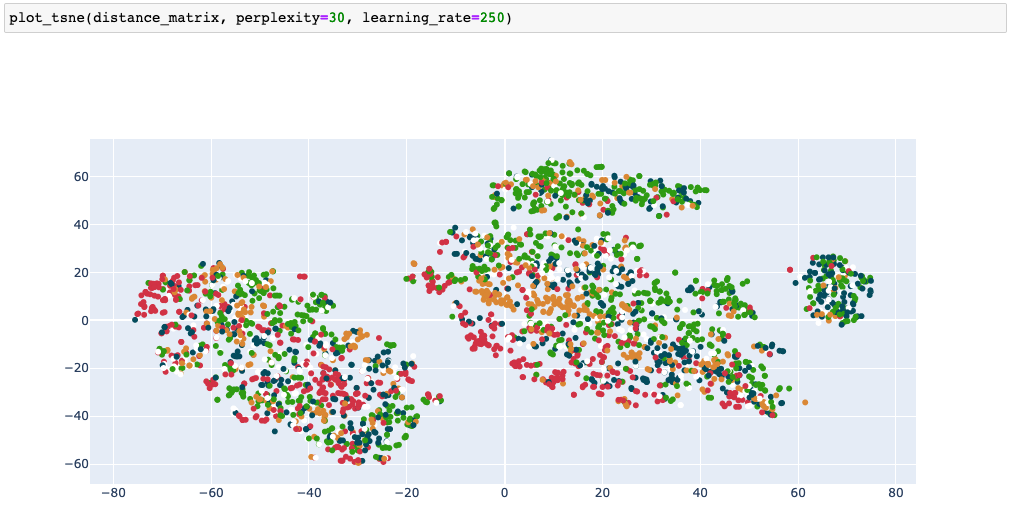
\includegraphics[width=\textwidth]{screenshots/pt_word_movers_distance_tsne1.png}
    \caption{Distance Matrix of the Word Mover's Distance with a pre-trained model (plotted with t-SNE)}
    \label{fig:wmd-pretrained-1}
  \end{center}
\end{figure}

% section analysis (end)